\chapter{Analyse de l’existant}
\section{Existant Organisationnel}
SPIE est un leader européen dans les domaines de l'énergie et des communications.

SPIE Sud-Est est présente en Auvergne, en Rhône-Alpes, en Provence-Alpes-Côte d'Azur et en Suisse.

Elle comporte trois spécialités~: 
\begin{itemize}
	\item transports et systèmes d'information~;
	\item industries~;
	\item génie climatique.\\
\end{itemize}

Les trois activités principales de l'entreprise sont \textbf{concevoir}, \textbf{réaliser} et \textbf{maintenir}.


SPIE souhaite \textbf{améliorer son processus de maintenance}. Dans cette optique, il est nécessaire pour notre équipe d'analyser l'existant organisationnel de cette entreprise.

\subsection{Structure organisationnelle de SPIE}
Penchons-nous sur l'étude des intervenants du processus de maintenance.

Les intervenants de ce processus sont~:
\begin{itemize}
\item le contrôle de gestion~;
\item les techniciens de maintenance~;
\item le responsable du contrat.\\
\end{itemize}

Voyons plus en détail quels sont les rôles de chacun de ces intervenants.

\paragraph{Contrôle de gestion}{Il assure la performance économique de l'entreprise et valide le reporting du responsable du contrat.}
\paragraph{Technicien de maintenance}{C'est la personne qui intervient directement sur le terrain pour effectuer la maintenance proprement dite. Il doit informer son supérieur des solutions qui ont été apportées à l'installation. Il doit également informer en cas de besoin en matériel (remplacement de matériel usagé par exemple).}
\paragraph{Responsable du contrat}{Sa mission principale est la gestion contractuelle. Il est également le responsable du \textit{reporting}, c'est-à-dire du compte-rendu permettant d'obtenir un bilan du projet à un moment particulier.}

Ces différents intervenants sont amenés à interagir, pour mener à bien le processus de maintenance.

La figure \vref{} présente les interactions entre les différents acteurs et services concernés dans le processus de maintenance.

\section{Processus stratégiques}

Le processus de gestion de contrats de maintenance et services est divis\'e en sept sous-processus.

\begin{itemize}
    \item Offre et revue d'offre
    \item Commande et revue de commande
    \item Lancements des prestation de service et travaux
    \item R\'ealisation de prestations de maintenances
    \item R\'ealisation travaux induits
    \item Evolution du contrat
    \item Solde de l'affaire et du contrat
\end{itemize}

\subsection{Offre et revue d'offre}

Le sous-processus Offre et revue d'offre se divise en etapes majeurs~:

\begin{itemize}
    \item On commance tout d'abort l'etudie des contrat potentiel a partir de processus commercial,
    processus tarvaux ou appel d'offre. Avant la prise de decision quand a la poursuite ou non,
    il est necessaire de recuperer l'ensemble des informations. Le processus peut s'arreter ici
    en cas d'abandon.
    \item Une reponse (d'une appel d'offre par exemple) est fournie au client potentiel simplement
    pour bute que SPIE entre officielement dans la course \'a une proposition d'une solution. Alors
    commence l'etude du chiffrage, choix et validation de la solution qui sera propos\'e au client.
    \item Ensuite, l'offre initiale est r\'ealiser en interne a partir de la solution choisie, puis
    valid\'e sous la responsabilit\'e du Pilote de l'Offre.
    \item Enfin cette offre initiale est envoy\'ee au client avec courrier d'accompagnement dans les
    Delais impartie.
\end{itemize}

\subsection{Commande et revue de commande}

Le sous-processus Commande et revue de commande est l'etape comporte l'etape importante de negociation
avec le client et se divise en etapes majeurs~:

\begin{itemize}
    \item L'offre est donc envoy\'ee au client, celle ci est alors enregistr\'e, diffus\'e puis le
    porteur attritr\'e est design\'e par le Responsable Activit\'e.
    \item Ensuite, pour pr\'epar\'e la negociation avec le client, arrive la commission de revue de
    commande puis validation des ecarts de negociation, plan d'action de validation.
    \item N\'egociation avec le client.
    \item Acceptation ou refus de la commande d\'efinitive tout juste n\'egoci\'ee avec le client.
    En cas de refus, le processus est alors abandonn\'e.
    \item Redaction et signature du contrat entre SPIE et le client.
\end{itemize}

\subsection{Lancements des prestation de service et travaux}

Le sous-processes Lancements des prestation de service et travaux se divise en etapes majeurs~:

\begin{itemize}
    \item Prise en compte du dossier contractuel et du dossier d'etude par le Responsable d'Affaire.
    \item Realisation du dossier complet et analyse r\'ealis\'ee.
    \item Arrive alors la r\'eunion  de lancement des prestation de service et travaux.
    \item Ensuite, vien a mobilisation des ressources pour la suite du projet, notament la cr\'eation
    des procedures et documents op\'erationnels, initialisation des syst\'emes de gestions.
    \item Enfin arriv\'ee de l'ecriture du rapport de l'\'etat des lieu chez le client puis sa prise en charge.
\end{itemize}

\subsection{R\'ealisation de prestations de maintenances}

Le sous-processes R\'ealisation de prestation de maintenances se divise en etapes majeurs mais a la difference
des pr\'ec\'edent, celles ci sont r\'ealis\'e de mani\`ere parall\'ele~:

\begin{itemize}
    \item Hexecutaion des travaux~;
    \item Maitrise \'economique et juridique du contrat~;
    \item Gestion des activit\'ees de reporting~;
    \item Revue periodique du contrat menant a une \'evolution des contrats.
\end{itemize}

\subsection{R\'ealisation travaux induits}

Pendant la dur\'ee du contratde maintenance, il est possible que le client ai besoin de travaux induits.
Ce sous processus est d\'edi\'e et divis\'es en etapes distinctes.

\begin{itemize}
    \item Le client va donc demander de mani\'ere exceptionnel la realisation des travaux induits a
    SPIE. Le cahier des charges va alors \'etre rediger. Il est possible que le sous processus soit
    abandoner ici. Sinon le cahier des charges est transmit \'a l'entit\'e travaux~;
    \item Si le contrat inclus les modalit'ees d'\'execution des travaux induits, alors le devis est
    automatiquement r\'edig\'e mais en d\'epense control\'e sinon deja present dans les closes du
    contrat client, valid\'e puis envoy\'e au client~;
    \item Sinon un devis est r\'edig\'e, valid\'e puis envoy\'e au client pour facturation~;
    \item Ensuite vien la pr\'eparation des travaux puis la r\'ealisation des prestations~;
    \item Viens en fait la facturation aupr\'es du service March\'e Gestion de la Garentie.
\end{itemize}

\subsection{Evolution du contrat}

L'evolution du contrat  est en faite un processus pouvant etre declancher soit par le client, soit
a l'initiative de SPIE pour proceder a une mise a jour de une ou plusieur closes du contrat client.
Elles comporte cependant une analyse de risque pour assurer la continuit\'e de la sant\'e de profits
de la companie sur ce contrat.


\subsection{Solde de l'affaire et du contrat}

Le sous-processus du solde de l'affaire et du contrat est r\'ealiser a la fin du contrat client. Celle
ci se deroule alors en plusieurs \'etape clef~:

\begin{itemize}
    \item Le contrat client, bilan d'affaire est revus, ainsi que les ecarts~;
    \item Alors arrive l'\'etape importante du solde des prestations et travaux a la reception des
    prestation achev\'ees. Ceci est realiser en consid\'erants les \'ecarts eventuelles entre les
    prestation et le contrat client initiale~;
    \item Viens ensuite l'\'etat des lieux de sortie chez le client si necessaire. Eventuellements,
    il peut avoir lieux d'un proces verbale en cas d'\'etat des lieux contradictoir~;
    \item La recette des prestations travaux \'etant effectu\'e, la gestion de la garentie est alors
    r\'ealis\'ee.
\end{itemize}

\section{Existant informatique}

\subsection{Cartographie applicative}

\begin{figure}[h]
    \centering
    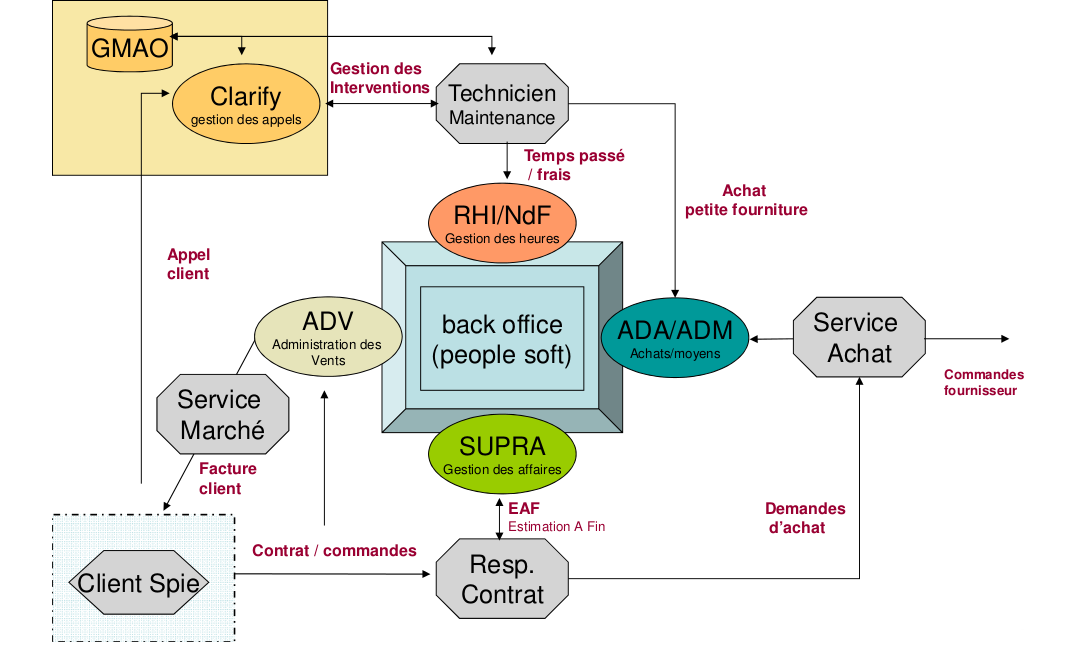
\includegraphics[width=140mm]{./images/cartographie_applicative.png}
    \caption{Cartographie applicative du système de gestion de contrats de maintenance de SPIE}
    \label{diagram:carto_app}
\end{figure}

\subsection{Description de l'architecture applicative}

Le système de gestion de contrats utilise 5 applications différentes :

%ADV : Administration des ventes
%ADA : Administration des achats
%ADM : Administration des moyens
%RHI : Relevé Hebdomadaire Individuel (Temps d'intervention des techniciens sur site)
%NdF : Note de Frais
%EAF : Estimation à fin (reste à faire)
%Clarify : Application de gestion des appels clients
%SUPRA : Application de gestion et suivi des affaires

\begin{itemize}
\item Clarify : Gestion des appels clients
\item RHI/NdF : Relevé Hebdomadaire Individuel / Note de frais
\item ADV : Administration des Ventes
\item ADA/ADM : Administration des Achats / Administration des moyens
\item SUPRA : Gestion et suivi des affaires
\end{itemize}


\subsubsection{Clarify}

Clarify est un outils de gestion des appels des clients. Lorsqu'un client appelle,  %TODO

\subsubsection{RHI/NdF}
\subsubsection{ADV}
\subsubsection{ADA/ADM}
\subsubsection{SUPRA}

\subsection{Améliorations possibles}

Nous pourrions penser à ajouter un dispositif nomade que les techniciens de SPIE puissent emporter avec eux lors de leurs opérations de maintenance. 
Ces appareils leurs permettraient par exemple :

\begin{itemize}
\item de se tenir à jour en temps réels de l'évolution des contrats
\item de remonter des problèmes rencontrés lors d'une opération de façon immédiate
\item d'enregistrer les nouvelles demandes du clients.
\item d'enregistrer les notes de frais
\item de rapporter leur temps d'intervention sur un site
\end{itemize}

\section{Dysfonctionnements}
